\chapter{Cahier des charges fonctionnel}

\section{Cahier des charges fonctionnel initial}
Les d\'eveloppeurs effectuent r\'eguli\`erement des calculs sur des flux de donn\'ees, ils ont besoins d'utilitaires simples et performants.
Notre but principal est d'offrir une alternative \`a la biblioth\`eque num-utils qui propose des utilitaires de calcul num\'erique. 
Cette biblioth\`eque est impl\'ement\'ee en Perl, l'adaptation en C devrait nous permettre d'obtenir de meilleures performances.
Voici le diagramme b\^ete \`a corne qui pr\'esente de fa\c con tr\`es g\'en\'erale le programme que nous devons livrer : 

\begin{figure}[h]
\begin{center}
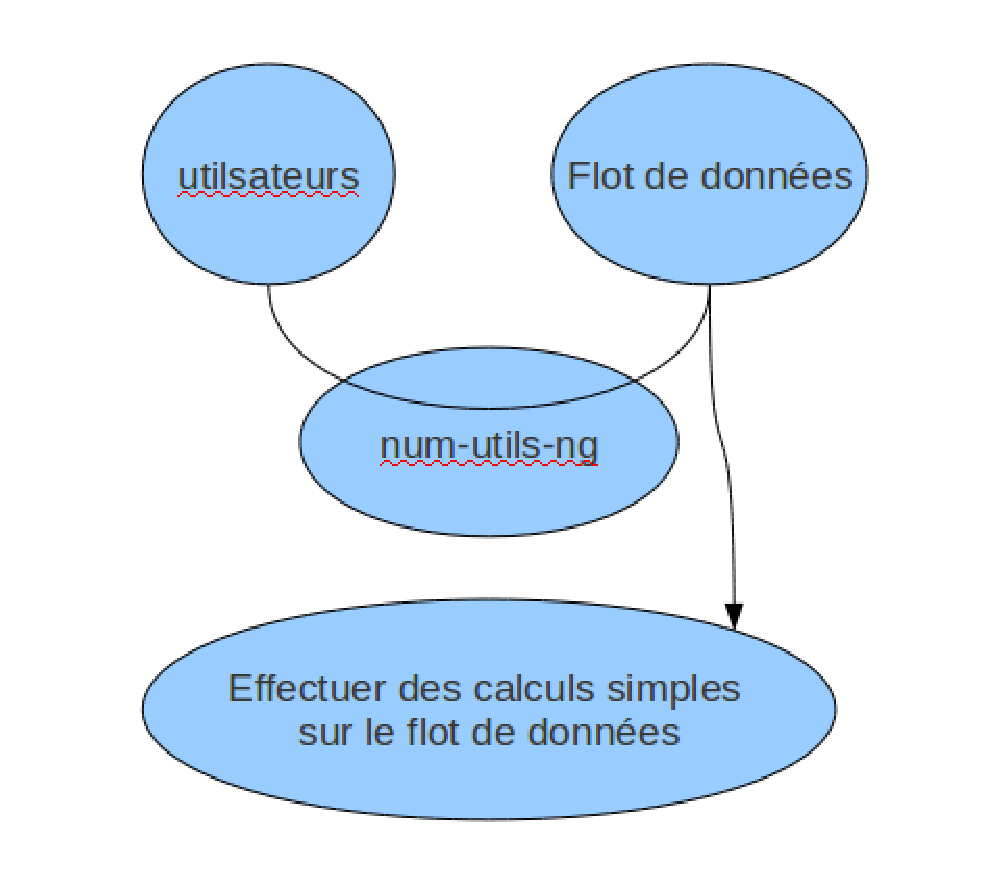
\includegraphics[width=9cm]{beteacorne.eps}
\end{center}
\caption{Diagramme B\^ete \`a cornes}
\label{fig:numprocess}
\end{figure}

Nous avons distingu\'e plusieurs fonctions contraintes pour notre biblioth\`eque : 
\newline
FP1 : Pouvoir effectuer des calculs simples sur des flots de donn\'ees.
\newline

FC1 : Les utilitaires propos\'es doivent \^etre plus rapide que les anciens.
\newline
FC2 : La biblioth\`eque doit \^etre pr\^ete sous un certain d\'elai.
\newline
FC3 : Cette biblioth\`eque doit \^etre \'ecrite dans un certain langage.
\newline
FC4 : Les programmes doivent \^etre libre.
\newline
FC5 : Les utilisateurs doivent pouvoir se servir facilement de ces utilitaires.
\newline
FC6 : La biblioth\`eque finale devra \^etre accessible  \`a tous.
\newline
FC7 : Il ne doit pas y avoir de bogues.
\newline


Les fonctions contraintes sont expos\'ees plus pr\'ecis\'ement dans le tableau fonctionnel ci-dessous.

\begin{table}[h]
\begin{center}
\begin{tabular}{|c|c|c|c|}
\hline
 & Crit\`ere & Niveau & Flexibilit\'e \\
\hline
 FC1 & Rapidit\'e & 10 fois plus rapide & 2 \\
\hline
 FC2 & D\'elai & 5 mois & 0 \\
\hline
 FC3 & Langage & C & 1 \\
\hline
 FC4 & Licence & GNU General Public License & 0 \\
\hline
 FC5 & Facilit\'e d'utilisation & M\^eme commandes qu'avant & 2 \\
\hline
 FC6 & Accessibilit\'e & Disponible sur le d\'ep\^ot officiel Debian & 1 \\
\hline
 FC7 & Nombre de bogues & 0 & 1 \\
\hline
\end{tabular}
\caption{Tableau Fonctionnel}
\end{center}
\label{tab:tabfonctionnel}
\end{table}

Flexibilit\'e : \newline
0 = imp\'eratif\newline
1 = peu n\'egociable\newline
2 = n\'egociable\newline
3 = tr\`es n\'egociable\newline

\section{Comparaison avec la version finale}
Nous voici \`a la fin de notre projet et d'une mani\`ere g\'en\'erale nous avons aboutit \`a une version op\'erationnelle de la biblioth\`eque mais nous 
allons maintenant voir si elle est conforme au cahier des charge que nous avions r\'edig\'e.

La fonction principale est bien entendu v\'erifi\'ee puisque nos utilitaires fonctionnent tous.

Prenons les fonctions contraintes une \`a une afin de v\'erifier si elles sont respect\'ees :

\begin{itemize}
\item [\textbullet] \textbf{FC1 : Les utilitaires propos\'es doivent \^etre plus rapides que les anciens.}
\newline
\normalsize
Nous avions esp\'er\'e aboutir \`a des programmes dix fois plus rapides que ceux de la version ant\'erieure mais cela n'a pas \'et\'e le cas : 
en moyenne nous atteignons des temps d'ex\'ecutions trois fois moins \'elev\'es. N\'eanmoins cette condition est n\'egociable et ne discr\'edite pas notre solution.
\item [\textbullet] \textbf{FC2 : La biblioth\`eque doit \^etre pr\^ete sous un certain d\'elai.}
\newline
\normalsize
Le d\'elai impos\'e de cinq mois a bien \'et\'e respect\'e.
\item [\textbullet] \textbf{FC3 : Cette biblioth\`eque doit \^etre \'ecrite dans un certain langage.}
\newline
\normalsize
Le langage C a bien \'et\'e utilis\'e et nous a permis un grand gain de vitesse.
\item [\textbullet] \textbf{FC4 : Les programmes doivent \^etre libre.}
\newline
\normalsize
La licence sous laquelle est diffus\'ee notre biblioth\`eque est GNU General Public License, ce crit\`ere est donc respect\'e.
\item [\textbullet] \textbf{FC5 : Les utilisateurs doivent pouvoir se servir facilement de ces utilitaires.}
\newline
\normalsize
Les commandes et options utilis\'ees sont exactement les m\^emes que dans la version ant\'erieure à l'exception des ``..'' remplac\'es par les `` : '' dans les expressions pour numrange et numrandom.
\item [\textbullet] \textbf{FC6 : La biblioth\`eque finale devra \^etre accessible  \`a tous.}
\newline
\normalsize
Le biblioth\`eque est disponible sur le d\'ep\^ot officiel Debian.
\item [\textbullet] \textbf{FC7 : Il ne doit pas y avoir de bogues.}
\newline
\normalsize
Il reste quelques bogues mineurs dont pour lesquels nous n'avons pas trouv\'es de solutions, ils r\'esultent pour la plupart d'un mauvaise utilisation des utilitaires propos\'es.
\end{itemize}

En conclusion on peut voir que la version finale de la biblioth\`eque est conforme au cahier des charges fonctionnels, notre solution est donc viable.